\begin{problemAllDefault}{Годинник на сканері}                                          


\noindent\begin{tabular}[t]{@{}p{0.72\textwidth}p{0.27\textwidth}@{}}
Секундна стрілка годинника переміщуєтся стрибками, тобто протягом секунди нерухома, а потім дуже швидко повертає на $\frac{1}{60}$ повного оберту. 
Стрілка являє собою тонкий відрізок довжини $d$~мм, що виходить з центру годинника.
\par
Годинник поклали на сканер, орієнтувавши звичайним чином (позначка ``12'' згори) й підібрали параметри сканування так, що:
&
{\ifnum\pdfoutput>0
\noindent\raisebox{-0.2\textwidth}{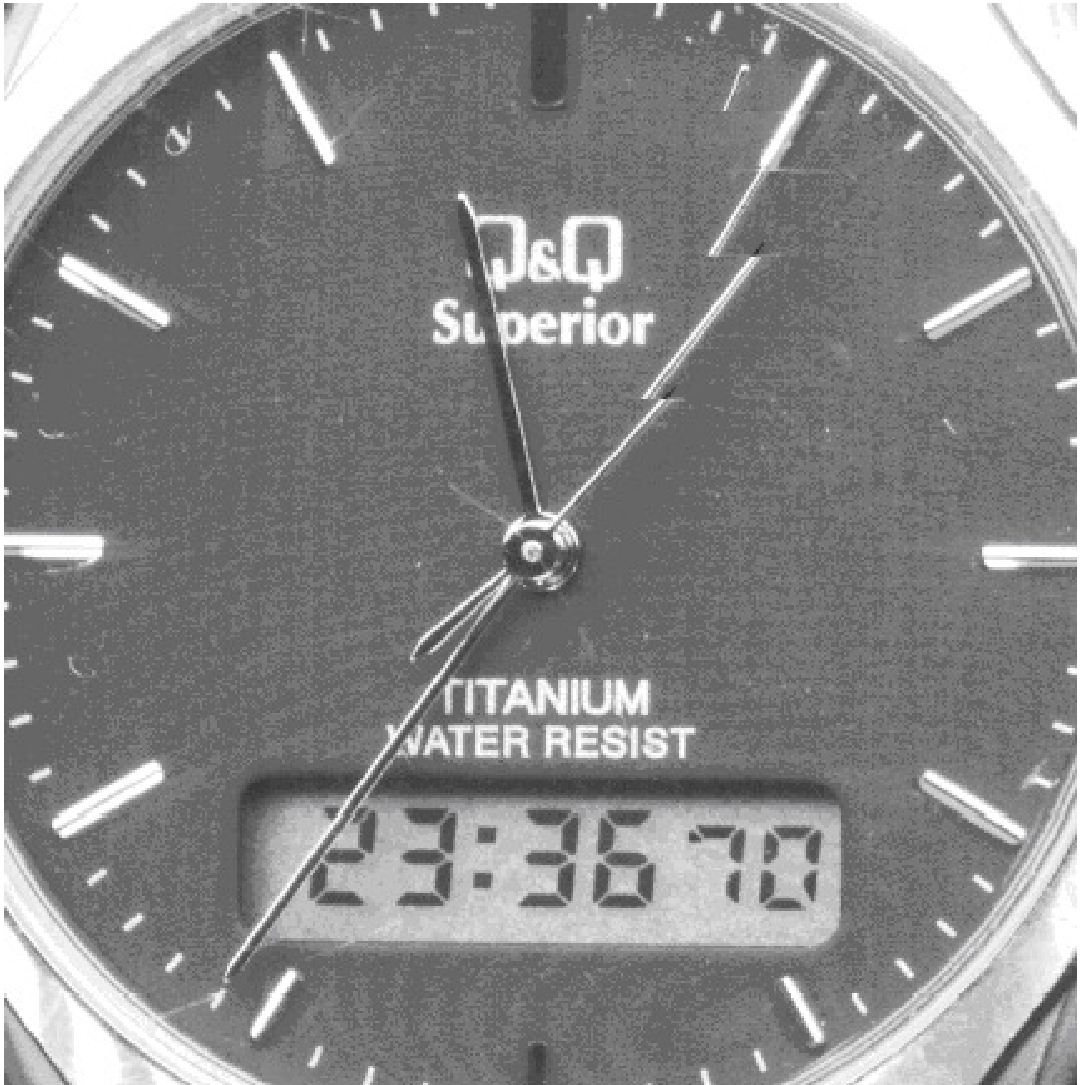
\includegraphics[width=0.25\textwidth,keepaspectratio=true]{watches_from_complex.pdf}}
\else
\begin{tiny}\colorbox{yellow}{Run not latex but pdflatex to insert picture}\par\end{tiny}
\begin{small}\colorbox{yellow}{Run not latex but pdflatex to insert picture}\end{small}
\ifnum\number\month > 7 \ERROR \fbox{Run not latex but pdflatex to insert picture}\fi
\fi}
\end{tabular}

\begin{enumerate}

\item
Сканування запускається відразу після того, як секундна стрілка виконала черговий стрибок і почала показувати $s$~секунд.

\item
Область сканування вибрана як квадрат розмірами ${2d\,\textnormal{мм}\times{}2d\,\textnormal{мм}}$, так, 
що вона в точності охоплює круг, який покриває секундна стрілка.

\item
Сканер за (кожну) 1~с встигає отримати прямокутне зображення висотою рівно $k$~мм 
(та шириною $2d$~мм, тобто в усю область сканування).

\item
Роздільча здатність сканера досить висока, щоб можна було знехтувати дискретністю 
зображень всер\'{е}дині кожної $k$-міліметрової смужки й рахувати відстані за звичайними геометричними формулами.

\end{enumerate}

Знайдіть сумарну довжину зображень секундної стрілки в отриманій картинці (зображення інших елементів годинника 
не~створюють проблем, бо секундна стрілка має зовсім інший колір).


\InputFile
Три цілі числа: $k$ (висота області, яку сканують за\nolinebreak[3] 1~с), 
$d$ (довжина стрілки) та 
$s$ (скільки секунд почала показувати стрілка у момент початку сканування.

${1\<k\<50}$,
${0.75k\<d\<100k}$,
відношення ${\frac{d}{k}}$ гарантовано не~є цілим числом,
${0\<s<60}$.


\OutputFile
Єдине дійсне число $l$\nolinebreak[3] --- сумарну довжину зображень секундної стрілки.

Відповідь буде зарахована, якщо відносна або абсолютна похибка (хоча~б одна з~них) не~перевищить $10^{-6}$.


\Example

\begin{example}
\exmp{36 90 10}{103.994544}%
\end{example}


\end{problemAllDefault}